% case name
\chapter{lock-exchange}
%
% - Purpose & Description:
%     These first two parts give reader short details about the test case,
%     the physical phenomena involved, the geometry and specify how the numerical solution will be validated
%
\section{Purpose}
%
This test demonstrates the ability of \telemac{3d} to model the motion
of two fluids with different densities.
%
\section{Description}
%
A 30~m long and 1.2~m wide tank with a constant water depth of 4~m is
considered.
This tank contains two fluids at rest with different densities because
of their salinity:
1~g/L in the left half part and 0~g/L on the right part.
The flow is governed by density effects.
The heavy fluid sinks below the lighter one by forming a saline wedge
which, according to the observations, makes an angle of about $\pi/3$
with the bottom [2].\\
The simulation is done with and without the hydrostatic hypothesis.
%
% - Reference:
%     This part gives the reference solution we are comparing to and
%     explicits the analytical solution when available;
%
% bibliography can be here or at the end
%\subsection{Reference}
%
%
\subsection{Reference}
%
[1] BARR D. Densimetric exchange flow in rectangular channels.
III. Large scale experiments. La Houille Blanche, 22, 619-632. 1967.

[2] BENJAMIN T. Gravity currents and related phenomena.
Journal of Fluid Mechanics, 31(2), 209-248. 1968.

[3] TURNER J. Buoyancy effects in fluids. Cambridge University Press.
1973.

[4] YIH C.S. Stratified flows. Academic Press. 1980.
%
% - Geometry and Mesh:
%     This part describes the mesh used in the computation
%
%
\subsection{Geometry and Mesh}
%
See Figure \ref{t3d:lock-exchange:mesh_CI}
%
\subsubsection{Bathymetry}
%
Flat bottom ($z$ = -4~m)
%
\subsubsection{Geometry}
%
Channel length = 30~m\\
Channel width = 1.2~m
%
\subsubsection{Mesh}
%
1,806 triangular elements\\
1,060 nodes\\
12 planes regularly spaced
%
\begin{figure} [H]
\centering
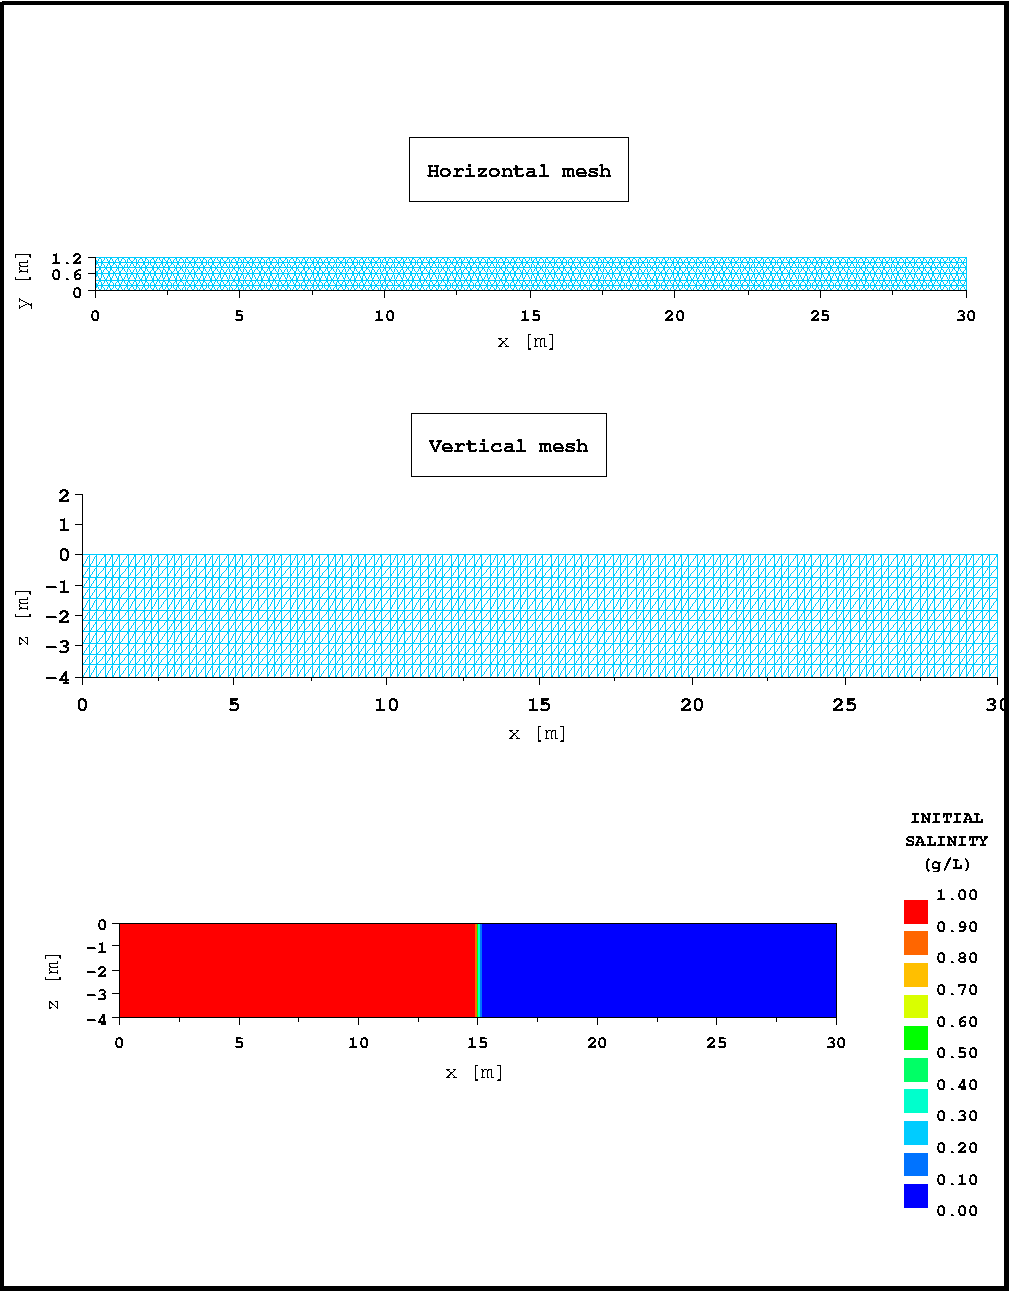
\includegraphics[scale=0.8]{../img/lock_exchange_mesh.pdf}
 \caption{Lock exchange test: Mesh and initial conditions for salinity}
 \label{t3d:lock-exchange:mesh_CI}
\end{figure}
%
% - Physical parameters:
%     This part specifies the physical parameters
%
%
\subsection{Physical parameters}
%
Diffusion: no\\
Density law depending on salinity:
\begin{equation}
\rho = \rho_{ref} (1 + 750.10^{-6} . sal ),
\rm{with } \rho_{ref} = 999.972~\rm{kg/m}^3
\end{equation}
Coriolis: no\\
Wind: no
%
% Experimental results (if needed)
%\subsection{Experimental results}
%
% bibliography can be here or at the end
%\subsection{Reference}
%
% Section for computational options
%\section{Computational options}
%
% - Initial and boundary conditions:
%     This part details both initial and boundary conditions used to simulate the case
%
%
\subsection{Initial and Boundary Conditions}
%
\subsubsection{Initial conditions}
%
Constant water depth = 4~m\\
No velocity\\
Initial salinity: 1~g/L on the left half part and 0~g/L in the other
part (defined in the subroutine \telfile{CONDIM} and the keyword
\telkey{INITIAL VALUES OF TRACERS})
%
\subsubsection{Boundary conditions}
%
Closed boundaries\\
No bottom friction
%
\subsection{General parameters}
%
Time step: 1~s\\
Simulation duration: 100~s
%
% - Numerical parameters:
%     This part is used to specify the numerical parameters used
%     (adaptive time step, mass-lumping when necessary...)
%
%
\subsection{Numerical parameters}
%
Hydrostatic and non-hydrostatic versions are run\\
Advection of velocities: N-type MURD scheme\\
Advection of tracers: PSI-type MURD scheme
%
\subsection{Comments}
%
% - Results:
%     We comment in this part the numerical results against the reference ones,
%     giving understanding keys and making assumptions when necessary.
%
%
\section{Results}
%
Figure \ref{t3d:lock-exchange:NH_res} presents the results obtained with
the non-hydrostatic version.

\begin{figure} [H]
\centering
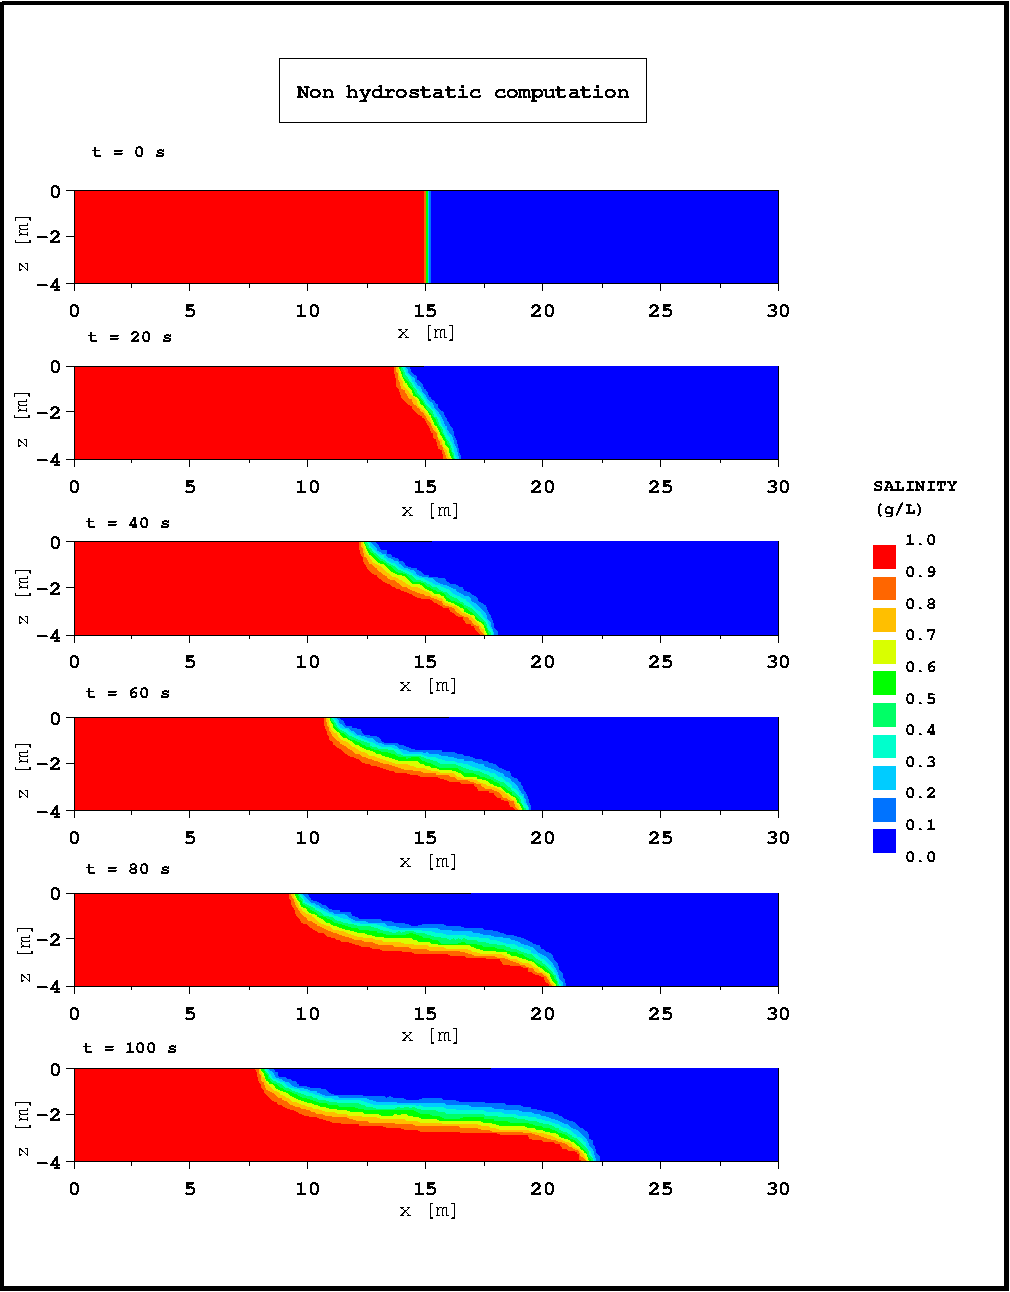
\includegraphics[scale=0.8]{../img/lock_exchange_NH_res.pdf}
 \caption{Lock exchange test: results from the non hydrostatic version}
 \label{t3d:lock-exchange:NH_res}
\end{figure}

The angle of $\pi/3$ between the front and the bottom is correctly
represented.\\
Considering that the whole potential energy of the initial conditions is
transformed into kinetic energy, it can be shown that the front velocity
is equal to 0.5 $\alpha$ where:
\begin{equation}
\alpha = \sqrt{g \frac{\rho_2-\rho_1}{\rho_2}h}
\end{equation}
The respective densities are $\rho_2$ = 1000.722~kg/m$^3$
and $\rho_1$ = 999.972~kg/m$^3$.
Then the theoretical velocity of the front is equal to 0.086~m/s.
The velocity computed by \telemac{3d} is approximately 0.07~m/s
(see figure \ref{t3d:lock-exchange:NH_res} where $\Delta x$ = 7~m
at $t$ = 100~s).
This underestimated result was predictable because the calculation is
started from a non-established situation with no velocity which makes
the calculation incorrect.\\
The results of the hydrostatic computation presented on figure
\ref{t3d:lock-exchange:hydro_res} show an average velocity of
approximately 0.065~m/s and an angle close to 90$^\circ$.

\begin{figure} [h]
\centering
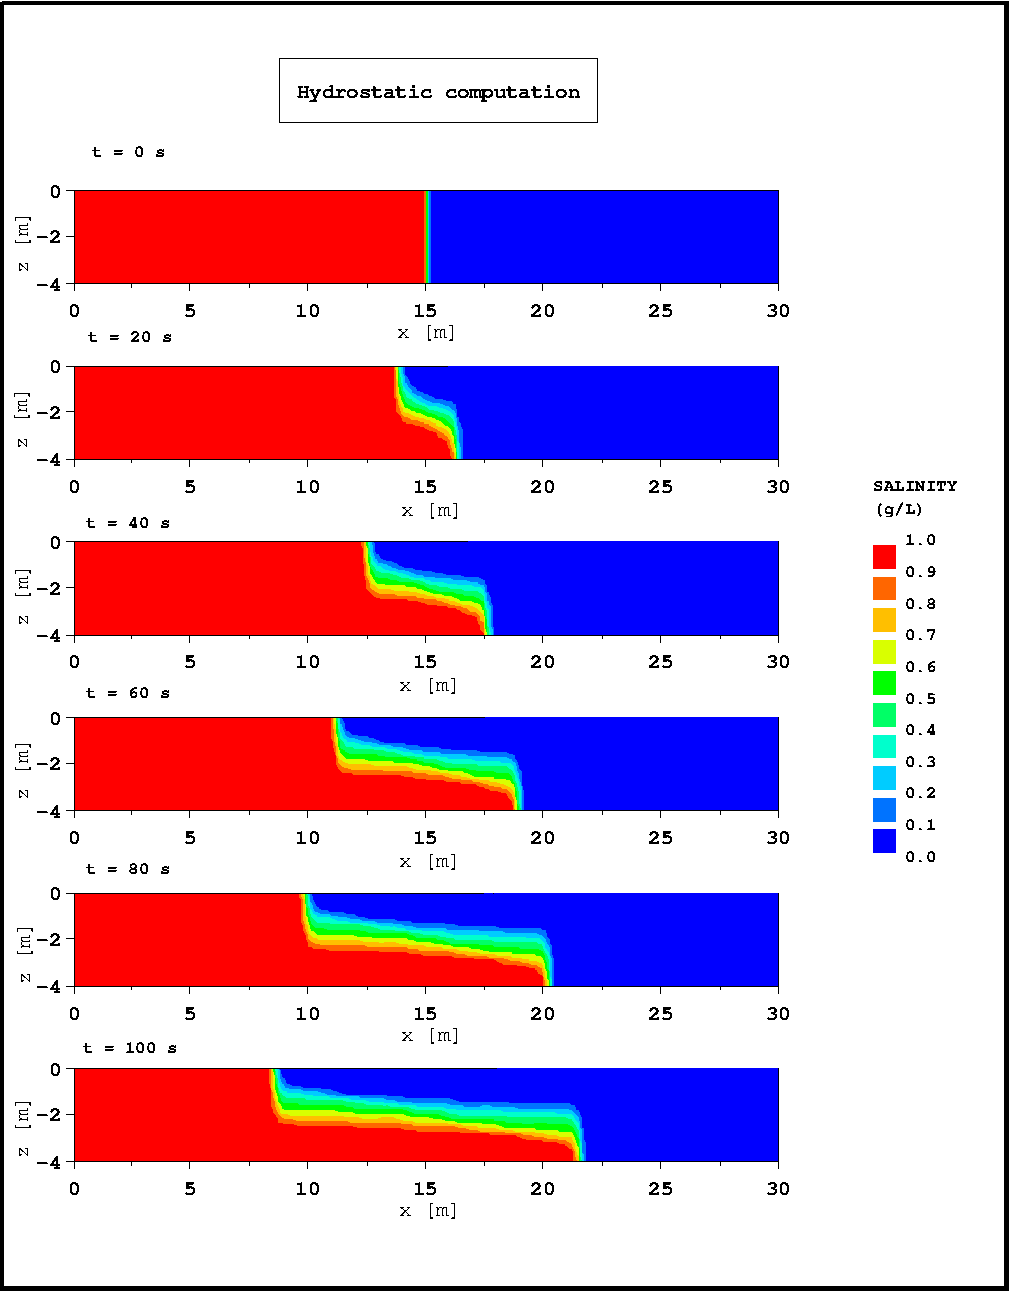
\includegraphics[scale=0.8]{../img/lock_exchange_hydro_res.pdf}
 \caption{Lock exchange test: results with the hydrostatic hypothesis}
 \label{t3d:lock-exchange:hydro_res}
\end{figure}

This shows that the hydrostatic hypothesis is not valid for this type of
computation.
%
\section{Conclusion}
%
\telemac{3d} simulates correctly the motion of fluids with different
densities.
%
% Here is an example of how to include the graph generated by validateTELEMAC.py
% They should be in test_case/img
%\begin{figure} [!h]
%\centering
%\includegraphics[scale=0.3]{../img/mygraph.png}
% \caption{mycaption}\label{mylabel}
%\end{figure}
%
% bibliography
%\section{Reference}
